Trabaje con la transformada unilateral $\mathcal L\{f\}(s)=\int_0^\infty e^{-st}f(t)\,dt$. Las funciones de entrada son causales. Use $H(t-a)=0$ para $t<a$ y $H(t-a)=1$ para $t\ge a$; sus valores aislados en saltos no alteran la transformada. Las gráficas continúan con el patrón indicado: $f$ alterna rampas de pendiente $1$ y mesetas, todas de duración $1$; $g$ repite su tramo de longitud $2$.
\begin{center}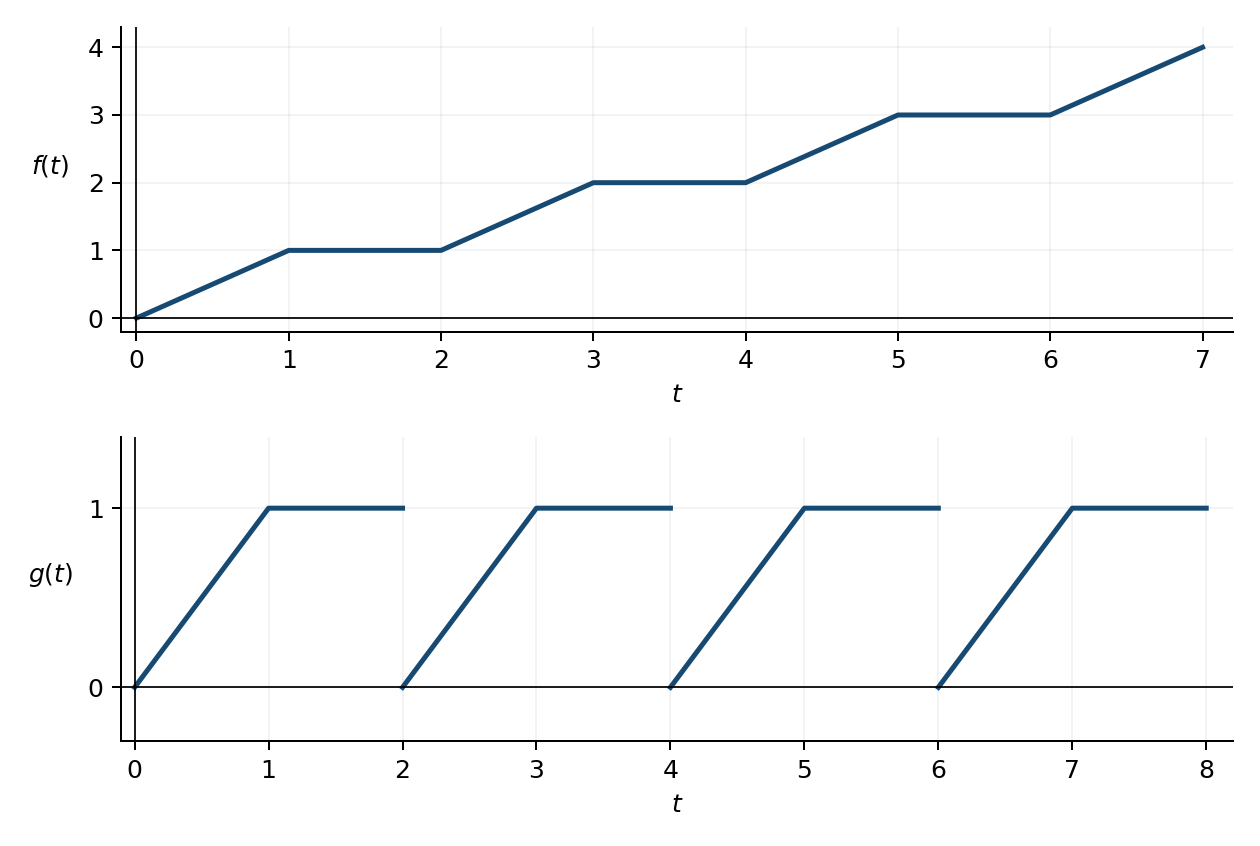
\includegraphics[width=.9\linewidth]{assets/M2-E0215-inputs.png}\end{center}

\begin{enumerate}[label=(\alph*),ref=\alph*,leftmargin=*]
\item Calcule $F(s)=\mathcal L\{f\}(s)$.
\item Resuelva por Laplace $y'+y=f(t)$, $y(0)=0$.
\item Calcule la transformada de la función periódica $g$.
\end{enumerate}
